% !TEX root = ../thesis.tex

\chapter{Introduction}
\label{chp:intro}

\section{Background and Motivation}

Legged robots have made remarkable strides in locomotion over the past
decade.  Quadrupeds such as the Unitree Go1, Spot (Boston Dynamics), and
ANYmal (ANYbotics) can now traverse challenging terrain, climb stairs, and
recover from perturbations using policies learned entirely in simulation via
deep reinforcement learning (RL)~\cite{lee2020learning,margolis2023walk}.
However, locomotion alone is insufficient for many real-world tasks: an
autonomous agent deployed in a factory, disaster site, or household must not
only \emph{move} but also \emph{interact} with its environment---picking up
objects, operating tools, or pressing switches.

Mounting a robotic arm on a legged platform creates a \emph{loco-manipulator}
that can both traverse and manipulate.  Yet the combination introduces
substantial control complexity.
The body dynamics of a walking quadruped couple with arm inertia, shifting
the centre of mass and generating reactive moments that disturb gait.
Conversely, locomotion oscillations perturb the arm end-effector.
Designing a controller that simultaneously achieves stable walking
\emph{and} accurate end-effector tracking is an open research challenge.

The Unitree B2+Z1 platform, comprising the B2 heavy-duty quadruped (approx.\
60\,kg, 12~leg DOFs) and the Z1 six-DOF robotic arm plus one gripper DOF,
is an industrial-grade loco-manipulator suited to this challenge.
The B2 offers greater payload capacity and locomotion robustness than the
lighter Go1, making it a more practical candidate for carrying a full 6-DOF
arm in real deployment.
This project investigates how a state-of-the-art decentralised multi-agent RL
framework can be adapted to the B2Z1 system, and what demonstration
capabilities can be established in simulation as a prerequisite for future
real-world experiments.

\section{Project Objectives}

The primary objectives of this project are:

\begin{enumerate}
  \item Adapt the open-source \textit{RoboDuet}
        framework~\cite{pan2024roboduet}---originally developed for the
        Unitree Go1+Z1 platform---to the Unitree B2+Z1 hardware.
  \item Load pre-trained arm and locomotion policies in the NVIDIA
        IsaacGym~\cite{makoviychuk2021isaac} physics simulator and verify
        their behaviour on B2Z1.
  \item Produce three reproducible simulation demonstrations:
        (a)~fixed-base arm manipulation,
        (b)~standing quadruped with simultaneous arm reaching, and
        (c)~a grasp-and-lift sequence with clearly visible object elevation.
  \item Characterise controller stability by measuring base height variation
        across all demonstration phases.
\end{enumerate}

\section{Task Definition and Project Pipeline}
\label{sec:task}

The task addressed in this project is formally defined as follows:

\begin{quote}
\textbf{Task.}\enspace Given the RoboDuet decentralised multi-agent RL
framework (originally developed for the Unitree Go1+Z1 platform) and
the Unitree B2+Z1 robot model, \emph{adapt the complete training and
control pipeline to the B2Z1 platform} and produce reproducible
simulation demonstrations of legged manipulation.
\end{quote}

\noindent
The project follows a four-stage pipeline, illustrated in
Figure~\ref{fig:pipeline}:

\begin{enumerate}
  \item \textbf{Platform Migration}
        (Chapter~\ref{chp:method}): replace the Go1+Z1 robot
        model with B2+Z1---URDF integration, 19-DOF indexing, PD gain
        recalibration ($K_p$: $35\!\to\!200$ for legs), and default pose
        update.
  \item \textbf{Simulation Setup}: configure IsaacGym with
        4096 parallel environments, domain randomisation (friction, mass,
        delay, external push), and a mixed-mode controller (torque for
        legs, position for arm).
  \item \textbf{Policy Training}: train two decoupled policies
        via PPO---a \emph{dog policy} $\pi_\text{dog}$ for locomotion
        stabilisation and an \emph{arm policy} $\pi_\text{arm}$ for
        spherical end-effector command tracking---through a two-stage
        curriculum (pre-training, then hybrid co-training; $\sim$200\,M
        environment steps).
  \item \textbf{Demonstration \& Evaluation}
        (Chapter~\ref{chp:results}): execute and evaluate three
        demonstrations of increasing complexity---fixed-base arm reaching,
        standing quadruped with arm reaching, and a complete
        grasp-and-lift sequence.
\end{enumerate}

\noindent
The success criteria are:
(a)~arm end-effector converges within 2\,cm of the commanded position;
(b)~base height remains within $\pm$3\,cm during free-standing
demonstrations; and
(c)~the grasp-and-lift demo achieves a visible lift of $\geq$10\,cm.

\begin{figure}[htbp]
  \centering
  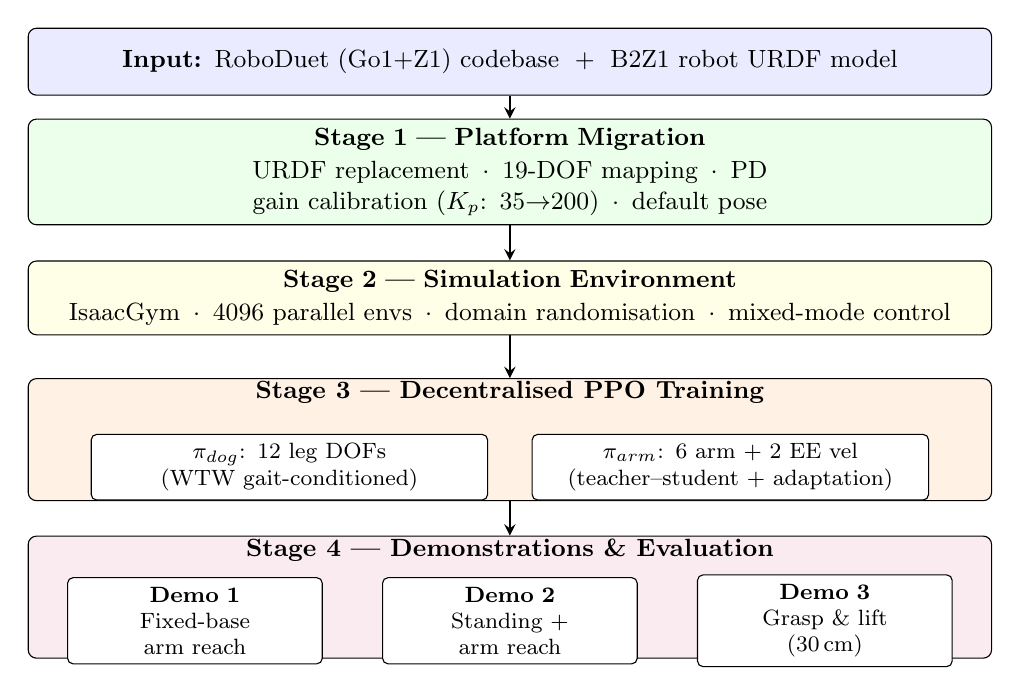
\begin{tikzpicture}[
      stage/.style={draw, rounded corners=3pt, text width=12cm,
                    minimum height=0.85cm, align=center, font=\small},
      sub/.style={draw, rounded corners=2pt, minimum height=0.55cm,
                  align=center, font=\footnotesize, fill=white},
      arr/.style={->,>=stealth,thick}
    ]
    \node[stage, fill=blue!8] (s0) at (0,0)
      {\textbf{Input:} RoboDuet (Go1+Z1) codebase \;$+$\;
       B2Z1 robot URDF model};
    \node[stage, fill=green!8] (s1) at (0,-1.4)
      {\textbf{Stage 1 --- Platform Migration}\\[1pt]
       URDF replacement \,$\cdot$\,
       19-DOF mapping \,$\cdot$\,
       PD gain calibration ($K_p$: 35$\to$200) \,$\cdot$\,
       default pose};
    \node[stage, fill=yellow!10] (s2) at (0,-3.0)
      {\textbf{Stage 2 --- Simulation Environment}\\[1pt]
       IsaacGym \,$\cdot$\,
       4096 parallel envs \,$\cdot$\,
       domain randomisation \,$\cdot$\,
       mixed-mode control};
    \node[stage, fill=orange!10, minimum height=1.55cm] (s3) at (0,-4.8) {};
    \node[font=\small\bfseries] at (0,-4.2)
      {Stage 3 --- Decentralised PPO Training};
    \node[sub, text width=4.8cm] at (-2.8,-5.15)
      {$\pi_\text{dog}$: 12 leg DOFs\\(WTW gait-conditioned)};
    \node[sub, text width=4.8cm] at ( 2.8,-5.15)
      {$\pi_\text{arm}$: 6 arm + 2 EE vel\\(teacher--student + adaptation)};
    \node[stage, fill=purple!8, minimum height=1.55cm] (s4) at (0,-6.8) {};
    \node[font=\small\bfseries] at (0,-6.2)
      {Stage 4 --- Demonstrations \& Evaluation};
    \node[sub, text width=3cm] at (-4,-7.1)
      {\textbf{Demo 1}\\Fixed-base\\arm reach};
    \node[sub, text width=3cm] at (0,-7.1)
      {\textbf{Demo 2}\\Standing +\\arm reach};
    \node[sub, text width=3cm] at (4,-7.1)
      {\textbf{Demo 3}\\Grasp \& lift\\(30\,cm)};
    \draw[arr] (s0) -- (s1);
    \draw[arr] (s1) -- (s2);
    \draw[arr] (s2) -- (s3);
    \draw[arr] (s3) -- (s4);
  \end{tikzpicture}
  \caption{End-to-end project pipeline.
           Stage~1 migrates the RoboDuet framework from Go1+Z1 to B2+Z1.
           Stage~2 configures GPU-accelerated simulation with domain
           randomisation.
           Stage~3 trains two decoupled policies via PPO.
           Stage~4 evaluates them through three progressively more complex
           demonstrations.}
  \label{fig:pipeline}
\end{figure}

\section{Individual Contributions}

This report describes individual work performed on the B2Z1
loco-manipulation project. The tasks undertaken and estimated individual
contribution percentages are summarised in Table~\ref{tab:contributions}.

\begin{table}[htbp]
  \centering
  \caption{Individual task contributions to the project.}
  \label{tab:contributions}
  \renewcommand{\arraystretch}{1.2}
  \begin{tabularx}{\textwidth}{lXr}
    \toprule
    \textbf{Task} & \textbf{Description} & \textbf{\%} \\
    \midrule
    Framework migration
      & Port RoboDuet configs (URDF, DOF mapping, PD gains) from Go1+Z1
        to B2+Z1; update \texttt{config\_go1.py}, \texttt{config\_asset.py},
        and \texttt{wtw\_config.py}.
      & 100 \\
    Control architecture analysis
      & Trace full 19-DOF indexing; identify gripper as DOF~18 outside the
        18-dim action space; determine mixed-mode (M) torque/position control
        split.
      & 100 \\
    Fixed-base arm demo
      & Implement and run \texttt{gen\_fixedbase\_arm.py}; produce
        \texttt{b2z1\_fixedbase\_arm.mp4}.
      & 100 \\
    Standing + reach demo
      & Implement \texttt{gen\_grab\_object.py}; identify arm policy forward
        reach direction via spherical command $(l,p,\psi)=(0.55,0.25,0)$;
        produce \texttt{b2z1\_grab\_object.mp4}.
      & 100 \\
    Grasp-and-lift demo (v7)
      & Design hybrid-lift box-teleport strategy; implement
        \texttt{gen\_grasp\_fixedbase\_success.py}; produce
        \texttt{b2z1\_grasp\_demo\_final.mp4} achieving 30\,cm lift
        with a 6\,cm green cube; fixed-base robot.
      & 100 \\
    Debugging iterations (v1--v6)
      & Identify root cause of backward arm reach in scripted-angle
        approach; validate policy-based approach; solve gripper DOF
        control bypass via direct state injection; develop hybrid
        XY-tracking + Z-animation lift strategy.
      & 100 \\
    \bottomrule
  \end{tabularx}
\end{table}

\section{Report Organisation}

Chapter~\ref{chp:related} reviews related work on RL-based legged
locomotion, robotic arm manipulation, and combined loco-manipulation.
Chapter~\ref{chp:method} describes the B2Z1 hardware, the RoboDuet
framework, and all technical details of the methodology.
Chapter~\ref{chp:results} presents the three demonstration results and
stability analysis.
Chapter~\ref{chp:conclusion} concludes with limitations and future work.
